% Created by tikzDevice version 0.10.1 on 2016-08-23 14:05:22
% !TEX encoding = UTF-8 Unicode
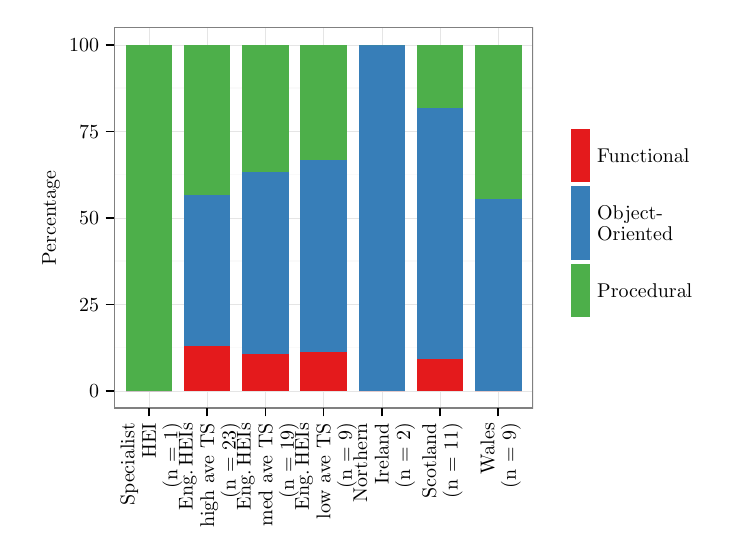
\begin{tikzpicture}[x=1pt,y=1pt]
\definecolor{fillColor}{RGB}{255,255,255}
\path[use as bounding box,fill=fillColor,fill opacity=0.00] (0,0) rectangle (252.94,180.67);
\begin{scope}
\path[clip] (  0.00,  0.00) rectangle (252.94,180.67);
\definecolor{drawColor}{RGB}{255,255,255}
\definecolor{fillColor}{RGB}{255,255,255}

\path[draw=drawColor,line width= 0.6pt,line join=round,line cap=round,fill=fillColor] (  0.00,  0.00) rectangle (252.94,180.68);
\end{scope}
\begin{scope}
\path[clip] ( 31.20, 43.19) rectangle (182.66,180.67);
\definecolor{fillColor}{RGB}{255,255,255}

\path[fill=fillColor] ( 31.20, 43.19) rectangle (182.66,180.67);
\definecolor{drawColor}{gray}{0.98}

\path[draw=drawColor,line width= 0.6pt,line join=round] ( 31.20, 65.06) --
	(182.66, 65.06);

\path[draw=drawColor,line width= 0.6pt,line join=round] ( 31.20, 96.31) --
	(182.66, 96.31);

\path[draw=drawColor,line width= 0.6pt,line join=round] ( 31.20,127.56) --
	(182.66,127.56);

\path[draw=drawColor,line width= 0.6pt,line join=round] ( 31.20,158.80) --
	(182.66,158.80);
\definecolor{drawColor}{gray}{0.90}

\path[draw=drawColor,line width= 0.2pt,line join=round] ( 31.20, 49.44) --
	(182.66, 49.44);

\path[draw=drawColor,line width= 0.2pt,line join=round] ( 31.20, 80.69) --
	(182.66, 80.69);

\path[draw=drawColor,line width= 0.2pt,line join=round] ( 31.20,111.93) --
	(182.66,111.93);

\path[draw=drawColor,line width= 0.2pt,line join=round] ( 31.20,143.18) --
	(182.66,143.18);

\path[draw=drawColor,line width= 0.2pt,line join=round] ( 31.20,174.43) --
	(182.66,174.43);

\path[draw=drawColor,line width= 0.2pt,line join=round] ( 43.82, 43.19) --
	( 43.82,180.67);

\path[draw=drawColor,line width= 0.2pt,line join=round] ( 64.86, 43.19) --
	( 64.86,180.67);

\path[draw=drawColor,line width= 0.2pt,line join=round] ( 85.90, 43.19) --
	( 85.90,180.67);

\path[draw=drawColor,line width= 0.2pt,line join=round] (106.93, 43.19) --
	(106.93,180.67);

\path[draw=drawColor,line width= 0.2pt,line join=round] (127.97, 43.19) --
	(127.97,180.67);

\path[draw=drawColor,line width= 0.2pt,line join=round] (149.01, 43.19) --
	(149.01,180.67);

\path[draw=drawColor,line width= 0.2pt,line join=round] (170.04, 43.19) --
	(170.04,180.67);
\definecolor{fillColor}{RGB}{228,26,28}

\path[fill=fillColor] ( 35.41, 49.44) rectangle ( 52.24, 49.44);
\definecolor{fillColor}{RGB}{55,126,184}

\path[fill=fillColor] ( 35.41, 49.44) rectangle ( 52.24, 49.44);
\definecolor{fillColor}{RGB}{77,175,74}

\path[fill=fillColor] ( 35.41, 49.44) rectangle ( 52.24,174.43);
\definecolor{fillColor}{RGB}{228,26,28}

\path[fill=fillColor] ( 56.45, 49.44) rectangle ( 73.27, 65.74);
\definecolor{fillColor}{RGB}{55,126,184}

\path[fill=fillColor] ( 56.45, 65.74) rectangle ( 73.27,120.08);
\definecolor{fillColor}{RGB}{77,175,74}

\path[fill=fillColor] ( 56.45,120.08) rectangle ( 73.27,174.43);
\definecolor{fillColor}{RGB}{228,26,28}

\path[fill=fillColor] ( 77.48, 49.44) rectangle ( 94.31, 62.60);
\definecolor{fillColor}{RGB}{55,126,184}

\path[fill=fillColor] ( 77.48, 62.60) rectangle ( 94.31,128.38);
\definecolor{fillColor}{RGB}{77,175,74}

\path[fill=fillColor] ( 77.48,128.38) rectangle ( 94.31,174.43);
\definecolor{fillColor}{RGB}{228,26,28}

\path[fill=fillColor] ( 98.52, 49.44) rectangle (115.35, 63.33);
\definecolor{fillColor}{RGB}{55,126,184}

\path[fill=fillColor] ( 98.52, 63.33) rectangle (115.35,132.76);
\definecolor{fillColor}{RGB}{77,175,74}

\path[fill=fillColor] ( 98.52,132.76) rectangle (115.35,174.43);
\definecolor{fillColor}{RGB}{228,26,28}

\path[fill=fillColor] (119.55, 49.44) rectangle (136.38, 49.44);
\definecolor{fillColor}{RGB}{55,126,184}

\path[fill=fillColor] (119.55, 49.44) rectangle (136.38,174.43);
\definecolor{fillColor}{RGB}{77,175,74}

\path[fill=fillColor] (119.55,174.43) rectangle (136.38,174.43);
\definecolor{fillColor}{RGB}{228,26,28}

\path[fill=fillColor] (140.59, 49.44) rectangle (157.42, 60.80);
\definecolor{fillColor}{RGB}{55,126,184}

\path[fill=fillColor] (140.59, 60.80) rectangle (157.42,151.70);
\definecolor{fillColor}{RGB}{77,175,74}

\path[fill=fillColor] (140.59,151.70) rectangle (157.42,174.43);
\definecolor{fillColor}{RGB}{228,26,28}

\path[fill=fillColor] (161.63, 49.44) rectangle (178.46, 49.44);
\definecolor{fillColor}{RGB}{55,126,184}

\path[fill=fillColor] (161.63, 49.44) rectangle (178.46,118.88);
\definecolor{fillColor}{RGB}{77,175,74}

\path[fill=fillColor] (161.63,118.88) rectangle (178.46,174.43);
\definecolor{drawColor}{gray}{0.50}

\path[draw=drawColor,line width= 0.6pt,line join=round,line cap=round] ( 31.20, 43.19) rectangle (182.66,180.67);
\end{scope}
\begin{scope}
\path[clip] (  0.00,  0.00) rectangle (252.94,180.67);
\definecolor{drawColor}{RGB}{0,0,0}

\node[text=drawColor,anchor=base east,inner sep=0pt, outer sep=0pt, scale=  0.72] at ( 25.80, 46.96) {0};

\node[text=drawColor,anchor=base east,inner sep=0pt, outer sep=0pt, scale=  0.72] at ( 25.80, 78.21) {25};

\node[text=drawColor,anchor=base east,inner sep=0pt, outer sep=0pt, scale=  0.72] at ( 25.80,109.45) {50};

\node[text=drawColor,anchor=base east,inner sep=0pt, outer sep=0pt, scale=  0.72] at ( 25.80,140.70) {75};

\node[text=drawColor,anchor=base east,inner sep=0pt, outer sep=0pt, scale=  0.72] at ( 25.80,171.95) {100};
\end{scope}
\begin{scope}
\path[clip] (  0.00,  0.00) rectangle (252.94,180.67);
\definecolor{drawColor}{RGB}{0,0,0}

\path[draw=drawColor,line width= 0.6pt,line join=round] ( 28.20, 49.44) --
	( 31.20, 49.44);

\path[draw=drawColor,line width= 0.6pt,line join=round] ( 28.20, 80.69) --
	( 31.20, 80.69);

\path[draw=drawColor,line width= 0.6pt,line join=round] ( 28.20,111.93) --
	( 31.20,111.93);

\path[draw=drawColor,line width= 0.6pt,line join=round] ( 28.20,143.18) --
	( 31.20,143.18);

\path[draw=drawColor,line width= 0.6pt,line join=round] ( 28.20,174.43) --
	( 31.20,174.43);
\end{scope}
\begin{scope}
\path[clip] (  0.00,  0.00) rectangle (252.94,180.67);
\definecolor{drawColor}{RGB}{0,0,0}

\path[draw=drawColor,line width= 0.6pt,line join=round] ( 43.82, 40.19) --
	( 43.82, 43.19);

\path[draw=drawColor,line width= 0.6pt,line join=round] ( 64.86, 40.19) --
	( 64.86, 43.19);

\path[draw=drawColor,line width= 0.6pt,line join=round] ( 85.90, 40.19) --
	( 85.90, 43.19);

\path[draw=drawColor,line width= 0.6pt,line join=round] (106.93, 40.19) --
	(106.93, 43.19);

\path[draw=drawColor,line width= 0.6pt,line join=round] (127.97, 40.19) --
	(127.97, 43.19);

\path[draw=drawColor,line width= 0.6pt,line join=round] (149.01, 40.19) --
	(149.01, 43.19);

\path[draw=drawColor,line width= 0.6pt,line join=round] (170.04, 40.19) --
	(170.04, 43.19);
\end{scope}
\begin{scope}
\path[clip] (  0.00,  0.00) rectangle (252.94,180.67);
\definecolor{drawColor}{RGB}{0,0,0}

\node[text=drawColor,rotate= 90.00,anchor=base east,inner sep=0pt, outer sep=0pt, scale=  0.72] at ( 38.53, 37.79) {Specialist};

\node[text=drawColor,rotate= 90.00,anchor=base east,inner sep=0pt, outer sep=0pt, scale=  0.72] at ( 46.30, 37.79) {HEI};

\node[text=drawColor,rotate= 90.00,anchor=base east,inner sep=0pt, outer sep=0pt, scale=  0.72] at ( 54.08, 37.79) {(n = 1)};

\node[text=drawColor,rotate= 90.00,anchor=base east,inner sep=0pt, outer sep=0pt, scale=  0.72] at ( 59.56, 37.79) {Eng.\,HEIs};

\node[text=drawColor,rotate= 90.00,anchor=base east,inner sep=0pt, outer sep=0pt, scale=  0.72] at ( 67.34, 37.79) {high ave TS};

\node[text=drawColor,rotate= 90.00,anchor=base east,inner sep=0pt, outer sep=0pt, scale=  0.72] at ( 75.12, 37.79) {(n = 23)};

\node[text=drawColor,rotate= 90.00,anchor=base east,inner sep=0pt, outer sep=0pt, scale=  0.72] at ( 80.60, 37.79) {Eng.\,HEIs};

\node[text=drawColor,rotate= 90.00,anchor=base east,inner sep=0pt, outer sep=0pt, scale=  0.72] at ( 88.38, 37.79) {med ave TS};

\node[text=drawColor,rotate= 90.00,anchor=base east,inner sep=0pt, outer sep=0pt, scale=  0.72] at ( 96.15, 37.79) {(n = 19)};

\node[text=drawColor,rotate= 90.00,anchor=base east,inner sep=0pt, outer sep=0pt, scale=  0.72] at (101.64, 37.79) {Eng.\,HEIs};

\node[text=drawColor,rotate= 90.00,anchor=base east,inner sep=0pt, outer sep=0pt, scale=  0.72] at (109.41, 37.79) {low ave TS};

\node[text=drawColor,rotate= 90.00,anchor=base east,inner sep=0pt, outer sep=0pt, scale=  0.72] at (117.19, 37.79) {(n = 9)};

\node[text=drawColor,rotate= 90.00,anchor=base east,inner sep=0pt, outer sep=0pt, scale=  0.72] at (122.67, 37.79) {Northern};

\node[text=drawColor,rotate= 90.00,anchor=base east,inner sep=0pt, outer sep=0pt, scale=  0.72] at (130.45, 37.79) {Ireland};

\node[text=drawColor,rotate= 90.00,anchor=base east,inner sep=0pt, outer sep=0pt, scale=  0.72] at (138.22, 37.79) {(n = 2)};

\node[text=drawColor,rotate= 90.00,anchor=base east,inner sep=0pt, outer sep=0pt, scale=  0.72] at (147.60, 37.79) {Scotland};

\node[text=drawColor,rotate= 90.00,anchor=base east,inner sep=0pt, outer sep=0pt, scale=  0.72] at (155.37, 37.79) {(n = 11)};

\node[text=drawColor,rotate= 90.00,anchor=base east,inner sep=0pt, outer sep=0pt, scale=  0.72] at (168.63, 37.79) {Wales};

\node[text=drawColor,rotate= 90.00,anchor=base east,inner sep=0pt, outer sep=0pt, scale=  0.72] at (176.41, 37.79) {(n = 9)};
\end{scope}
\begin{scope}
\path[clip] (  0.00,  0.00) rectangle (252.94,180.67);
\definecolor{drawColor}{RGB}{0,0,0}

\node[text=drawColor,rotate= 90.00,anchor=base,inner sep=0pt, outer sep=0pt, scale=  0.72] at ( 10.20,111.93) {Percentage};
\end{scope}
\begin{scope}
\path[clip] (  0.00,  0.00) rectangle (252.94,180.67);
\definecolor{fillColor}{RGB}{255,255,255}

\path[fill=fillColor] (191.20, 71.20) rectangle (244.41,152.66);
\end{scope}
\begin{scope}
\path[clip] (  0.00,  0.00) rectangle (252.94,180.67);
\definecolor{fillColor}{RGB}{228,26,28}

\path[fill=fillColor] (196.18,124.98) rectangle (203.29,144.07);
\end{scope}
\begin{scope}
\path[clip] (  0.00,  0.00) rectangle (252.94,180.67);
\definecolor{fillColor}{RGB}{55,126,184}

\path[fill=fillColor] (196.18, 96.69) rectangle (203.29,123.56);
\end{scope}
\begin{scope}
\path[clip] (  0.00,  0.00) rectangle (252.94,180.67);
\definecolor{fillColor}{RGB}{77,175,74}

\path[fill=fillColor] (196.18, 76.18) rectangle (203.29, 95.27);
\end{scope}
\begin{scope}
\path[clip] (  0.00,  0.00) rectangle (252.94,180.67);
\definecolor{drawColor}{RGB}{0,0,0}

\node[text=drawColor,anchor=base west,inner sep=0pt, outer sep=0pt, scale=  0.72] at (205.81,139.82) {};

\node[text=drawColor,anchor=base west,inner sep=0pt, outer sep=0pt, scale=  0.72] at (205.81,132.05) {Functional};

\node[text=drawColor,anchor=base west,inner sep=0pt, outer sep=0pt, scale=  0.72] at (205.81,124.27) {};
\end{scope}
\begin{scope}
\path[clip] (  0.00,  0.00) rectangle (252.94,180.67);
\definecolor{drawColor}{RGB}{0,0,0}

\node[text=drawColor,anchor=base west,inner sep=0pt, outer sep=0pt, scale=  0.72] at (205.81,119.31) {};

\node[text=drawColor,anchor=base west,inner sep=0pt, outer sep=0pt, scale=  0.72] at (205.81,111.53) {Object-};

\node[text=drawColor,anchor=base west,inner sep=0pt, outer sep=0pt, scale=  0.72] at (205.81,103.76) {Oriented};

\node[text=drawColor,anchor=base west,inner sep=0pt, outer sep=0pt, scale=  0.72] at (205.81, 95.98) {};
\end{scope}
\begin{scope}
\path[clip] (  0.00,  0.00) rectangle (252.94,180.67);
\definecolor{drawColor}{RGB}{0,0,0}

\node[text=drawColor,anchor=base west,inner sep=0pt, outer sep=0pt, scale=  0.72] at (205.81, 91.02) {};

\node[text=drawColor,anchor=base west,inner sep=0pt, outer sep=0pt, scale=  0.72] at (205.81, 83.25) {Procedural};

\node[text=drawColor,anchor=base west,inner sep=0pt, outer sep=0pt, scale=  0.72] at (205.81, 75.47) {};
\end{scope}
\end{tikzpicture}
